\subsection{Пример работы алгоритма}
\par Для примера рассмотрим следующий граф $G$ (рис.~\ref{fig:picg}).

\begin{figure}[h]
	\begin{center}
	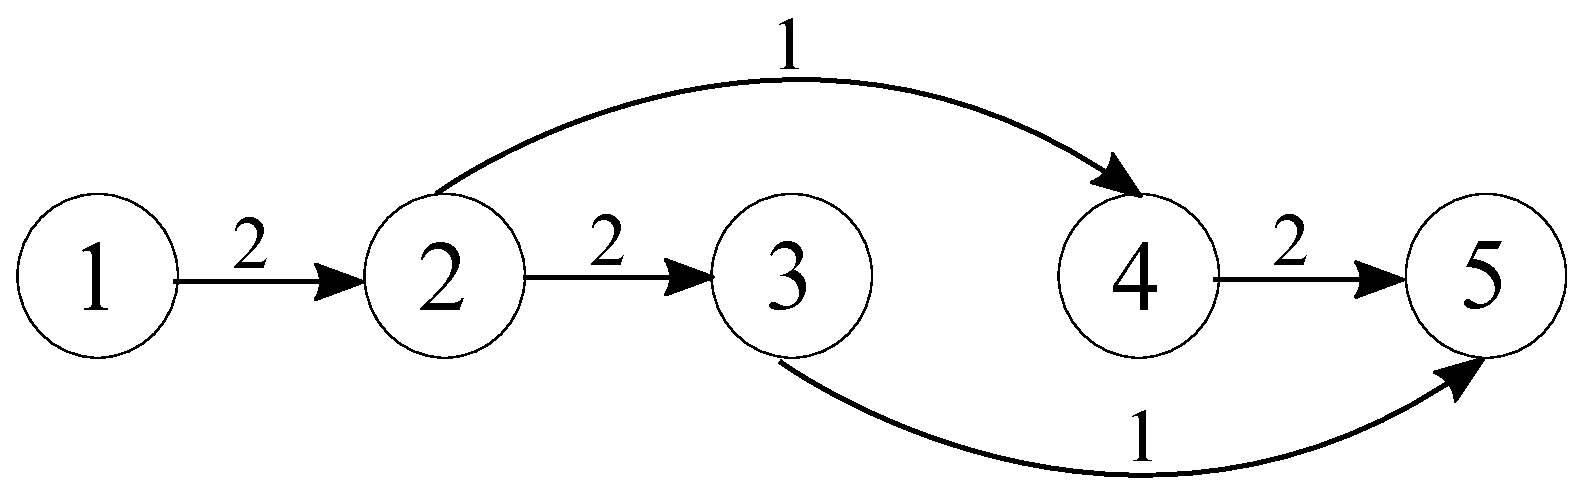
\includegraphics[width=0.9\textwidth]{example1}
	\end{center}
	\caption{Граф $G$.}
	\label{fig:picg}
\end{figure}
\par Для этого графа $X = \{1, 2, 3, 4, 5\}$, $C = \{1, 2\}$. Этот граф не имеет кратных дуг, поэтому их можно представлять как пары $(x, y)$ вершин графа, где $x$ -- начало дуги, $y$ -- её конец. Каждая дуга допускает ровно один цвет, надписанный над ней. Таким образом, $U =\{(1, 2), (2, 3), (2, 4), (3, 5), (4, 5)\}$, $U_1 =\{(2, 4), (3, 5)\}$, $U_2 =\{(1, 2), (2, 3), (4, 5)\}$. Непосредственно можно убедиться, что граф $G$ не содержит контуров, а его вершины топологически упорядочены.
\par Пусть $s = 1$, $t = 5$, а стохастическая матрица $P$ имеет вид:
\[P = \begin{pmatrix} 
0,7 & 0,3\\ 
0,3 & 0,7 
\end{pmatrix}
\]
\par Применяя вышеизложенный алгоритм, найдём матрицу вероятностей $P^{(1)}$ для вершины $s = 1$, а также стратегию $(v_{i, n})_{1 \le n < 5, i = 1, 2}$.
\par Для вершины $5$ имеем:
\[P^{(5)} = E = \begin{pmatrix} 
1 & 0\\ 
0 & 1 
\end{pmatrix}
\]
\par Для дальнейшего нам понадобится одно обозначение.
\par Будем обозначать $L_k(A)$ взятие $k$-й строки матрицы $A$, т.е. 
\[L_k((a_{i,j})_{i,j = 1}^{M}) = (a_{k, 1}, a_{k, 2}, ..., a_{k, M}).\]
\par Из определения умножения матриц следует, что:
\[
L_k(A \cdot B) = L_k(A) \cdot B.
\]
\par Для вершины $4$ имеем $X_1(4) = \emptyset$, поэтому $v_{1, 4} = \bigotimes$.
\par $X_2(4) = \{5\}$, поэтому: 
\[L_2(P^{(4, 5)}) = L_2(P) \cdot P^{(5)} = \begin{pmatrix} 0,3 & 0,7 \end{pmatrix} \begin{pmatrix} 1 & 0\\ 0 & 1 \end{pmatrix} = \begin{pmatrix} 0,3 & 0,7 \end{pmatrix} \]
\par Здесь $v_{2, 4} = 5$ как единственная вершина множества $X_2(4)$.
\par Таким образом, 
\[
P^{(4)} = \begin{pmatrix} 0 & 0\\ 0,3 & 0,7 \end{pmatrix}.
\]

\par Для вершины $3$ имеем $X_1(3) = \{5\}$, поэтому: 
\[L_1(P^{(3, 5)}) = L_1(P) \cdot P^{(5)} = \begin{pmatrix} 0,7 & 0,3 \end{pmatrix} \begin{pmatrix} 1 & 0\\ 0 & 1 \end{pmatrix} = \begin{pmatrix} 0,7 & 0,3 \end{pmatrix} \]
\par Здесь $v_{1, 3} = 5$ как единственная вершина множества $X_1(3)$.
\par $X_2(3) = \emptyset$, поэтому $v_{2, 3} = \bigotimes$.
\par Таким образом, 
\[
P^{(3)} = \begin{pmatrix} 0,7 & 0,3\\ 0 & 0 \end{pmatrix}.
\]

\par Для вершины $2$ имеем $X_1(2) = \{4\}$, поэтому: 
\[L_1(P^{(2, 4)}) = L_1(P) \cdot P^{(4)} = \begin{pmatrix} 0,7 & 0,3 \end{pmatrix} \begin{pmatrix} 0 & 0\\ 0,3 & 0,7 \end{pmatrix} = \begin{pmatrix} 0,09 & 0,21 \end{pmatrix} \]
\par Здесь $v_{1, 2} = 4$ как единственная вершина множества $X_1(2)$.
\par $X_2(2) = \{3\}$, поэтому: 
\[L_2(P^{(2, 3)}) = L_2(P) \cdot P^{(3)} = \begin{pmatrix} 0,3 & 0,7 \end{pmatrix} \begin{pmatrix} 0,7 & 0,3\\ 0 & 0 \end{pmatrix} = \begin{pmatrix} 0,21 & 0,09 \end{pmatrix} \]
\par Здесь $v_{2, 2} = 3$ как единственная вершина множества $X_2(2)$.
\par Таким образом, 
\[
P^{(2)} = \begin{pmatrix} 0,09 & 0,21\\ 0,21 & 0,09 \end{pmatrix}.
\]

\par Для вершины $1$ имеем $X_1(1) = \emptyset$, поэтому $v_{1, 1} = \bigotimes$.
\par $X_2(1) = \{2\}$, поэтому: 
\[L_2(P^{(1, 2)}) = L_2(P) \cdot P^{(2)} = \begin{pmatrix} 0,3 & 0,7 \end{pmatrix} \begin{pmatrix} 0,09 & 0,21\\ 0,21 & 0,09 \end{pmatrix} = \begin{pmatrix} 0,174 & 0,126 \end{pmatrix} \]
\par Здесь $v_{2, 1} = 2$ как единственная вершина множества $X_2(1)$.
\par Таким образом, 
\[
P^{(1)} = \begin{pmatrix} 0 & 0\\ 0,174 & 0,126 \end{pmatrix}.
\]
\par Как мы видим, в случае, если путешественник находится в стартовой вершине в цвете $1$, он не сможет достичь вершины $5$ ни при каком условии: $p_1 = 0$. Если же он изначально находится в цвете $2$, он может достичь вершины $5$ с вероятностью $p_2 = 0,174 + 0,126 = 0,3$. Найденные вершины стратегии укажут путешественнику наиболее оптимальный маршрут.